%!TEX root = ../coursework.tex

\section{SAT-задачи в криптоанализе}

\label{sec:sat-crypto}

Задача булевой выполнимости (SAT) спрашивает, существует ли присваивание булевых переменных, удовлетворяющее всем клаузам формулы в конъюнктивной нормальной форме (CNF). В криптоанализе это естественная унификация: ключ, промежуточные состояния и побитовые зависимости между открытым и шифртекстом моделируются как система булевых ограничений; валидное присваивание соответствует искомому секрету \cite{Zhang2000}.

Логический криптоанализ формулирует атаку как SAT‑инстанс и решает его общим решателем. Классические вехи: редукция DES к SAT‑формуле (десятки тысяч переменных, порядка миллиона клауз) \cite{Zhang2000} и последующие работы, где SAT применялся для:
\begin{itemize}
  \item поиска прообразов и коллизий в хэш‑функциях \cite{Mironov2006};
  \item восстановления ключей для облегчённых раундовых конфигураций блочных шифров (в~т.~ч. легковесных) \cite{Lafitte2014};
  \item автоматизированного поиска дифференциальных и линейных трейлов.
\end{itemize}

Практическая применимость обеспечена прогрессом CDCL‑решателей (обучение по конфликтам, эвристики ветвления и выбора фаз, рестарты, вивификация клауз, препроцессинг) и специализированной поддержкой XOR‑ограничений (исключение Гаусса «на лету», SAT+XOR‑ядра в~CryptoMiniSat и др.) \cite{Im2025}.

Алгоритм шифрования разворачивается в битовую схему:
\begin{itemize}
  \item линейные над \(\mathbb{F}_2\) зависимости (XOR) либо сохраняются отдельным типом ограничения (если решатель это поддерживает), либо переводятся в CNF через вспомогательные переменные;
  \item нелинейности (S‑блоки) заменяются на компактные логические сети с оптимизированными CNF‑кодировками или табличными энкодингами;
  \item дополнительные структурные ограничения (раундовые ключи, известные/частично известные биты) добавляются как унарные/бинарные клаузы.
\end{itemize}

Для кардинальных/псевдобулевых ограничений применяются стандартные энкодинги «ровно/не больше \(t\)»:
\begin{itemize}
  \item последовательные счётчики (Sequential counter) — хорошие свойства unit‑propagation; размер растёт с \(n\) и \(t\);
  \item тотализаторы (Totalizer) — сильное распространение единиц, особенно при малых \(t\);
  \item аддерные (Adder) и бинарные схемы — умеренный размер и удобство для инкрементального SAT;
  \item сортировочные сети — более крупные по числу клауз, но с хорошей локальностью;
  \item PB‑подходы — прямая поддержка ограничений вида \(\sum w_i x_i \le t\) с последующей CNF‑компиляцией.
\end{itemize}

В результате получается крупная, но структурированная формула; в ряде решателей (напр., CryptoMiniSat) можно смешивать CNF с XOR‑блоками, а при отсутствии нативной поддержки XOR ограничения компилируют в CNF \cite{Im2025}.

\subsection*{Кодовые схемы (Мак‑Элис): синдром и вес}
Для кодовых криптосистем редукция ещё чище. Пусть опубликована \(H \in \{0,1\}^{(n-k)\times n}\) и дан синдром \(s\). Задача: найти \(e \in \{0,1\}^n\) веса \(\mathrm{wt}(e)=t\):
\[
H e^{\top} = s^{\top} \quad \text{над } \mathbb{F}_2.
\]
Каждая строка \(H\) даёт XOR‑ограничение, а \(\mathrm{wt}(e)=t\) кодируется кардинальным энкодингом (либо «ровно \(t\)», либо «не больше \(t\)» с доведением до равенства). В терминах SAT это «найти подмножество позиций мощности \(t\)» с заданными паритетами — эквивалент задачи декодирования на ограниченном расстоянии. Такой SAT‑подход — частный случай алгебраического криптоанализа над \(\mathbb{F}_2\), где решатель выступает универсальным механизмом вывода следствий (смешение линейной и булевой логики) \cite{Zhang2000,Lafitte2014}.

\subsection*{Ограничения SAT‑подхода в полноразмерных параметрах}
\begin{enumerate}
  \item Для типичных параметров Classic McEliece (например, \(n=8192,\, t=128\)) одна только кардинальность влечёт тысячи вспомогательных переменных и сотни тысяч/миллионы клауз; комбинаторное пространство \(\binom{n}{t}\) астрономично.
  \item Матрицы Гоппы, как правило, не формируют выраженного «хребта» (\textit{backbone}) — множества переменных, принимающих одинаковые значения во всех допустимых решениях, что обычно облегчает работу CDCL. Вследствие этого переносимость обученных клауз ограничена, а многочисленные XOR‑ограничения требуют ресурсоёмкого линейного вывода.
  \item Высокая арность XOR и плотные соединения ухудшают локальность, увеличивая длину вывода и снижая эффективность стандартных эвристик ветвления \cite{Im2025}.
\end{enumerate}

\begin{figure}[t]
  \centering
  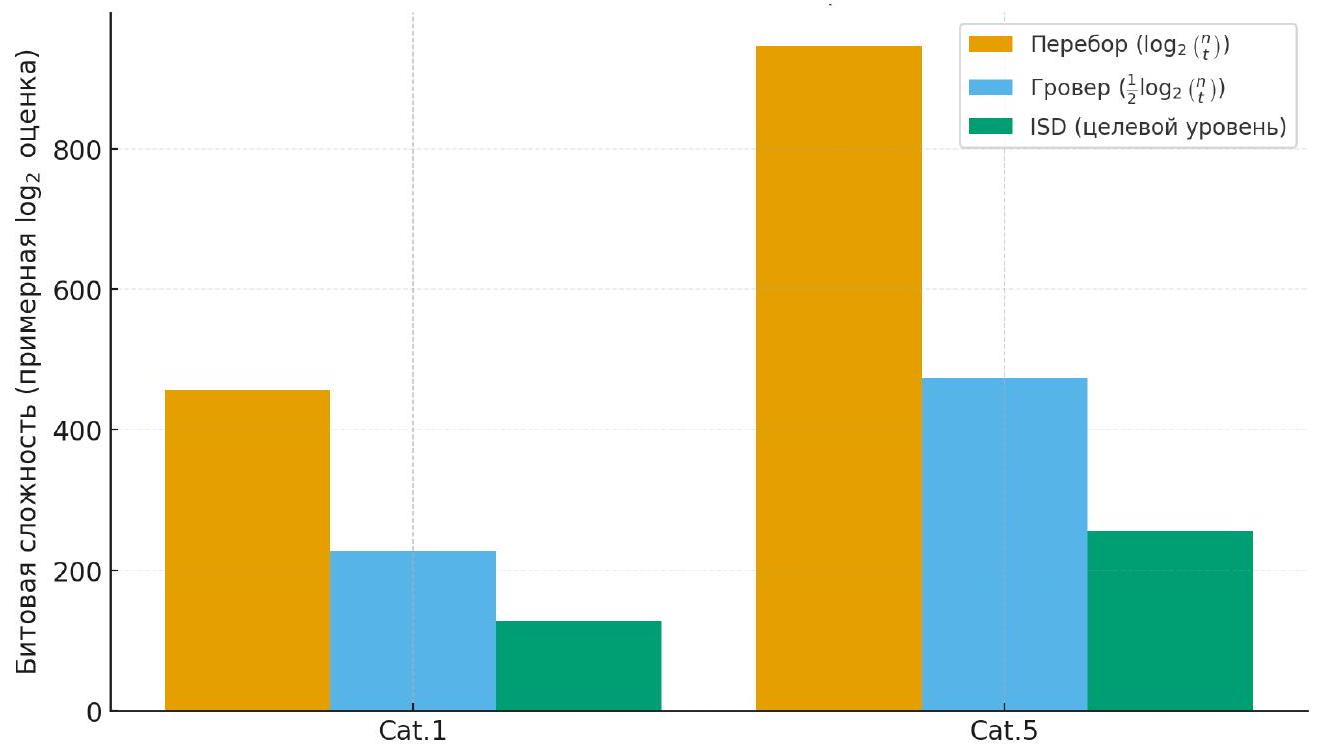
\includegraphics[width=\textwidth]{2025_09_09_2d30ddf39efcfb4865a0g-10}
  \caption{Сопоставление оценок сложности атак \cite{Grover1996}.}
  \label{fig:attack-complexity}
\end{figure}

SAT‑решатели практически применимы на урезанных параметрах (для калибровки сложности, прототипирования гибридных атак, проверки идей) \cite{Sirdey2023}, но не конкурируют с лучшими семействами алгоритмов ISD на полномасштабных инстансах.

Именно здесь возникает мотивация для квантовых оптимизаторов: перевод SAT/XOR‑PB формулировок в QUBO/модель Изинга позволяет задействовать квантовый отжиг и родственные методы как поисковые решатели в больших дискретных пространствах \cite{Bian2018,Pei2025}.
